\documentclass{article}
\usepackage{fontspec,tikz,graphicx}
\setmainfont{Times New Roman}
\usepackage[a3paper,margin=1cm]{geometry}
\pagestyle{empty}
\begin{document}
\noindent\resizebox{\textwidth}{!}{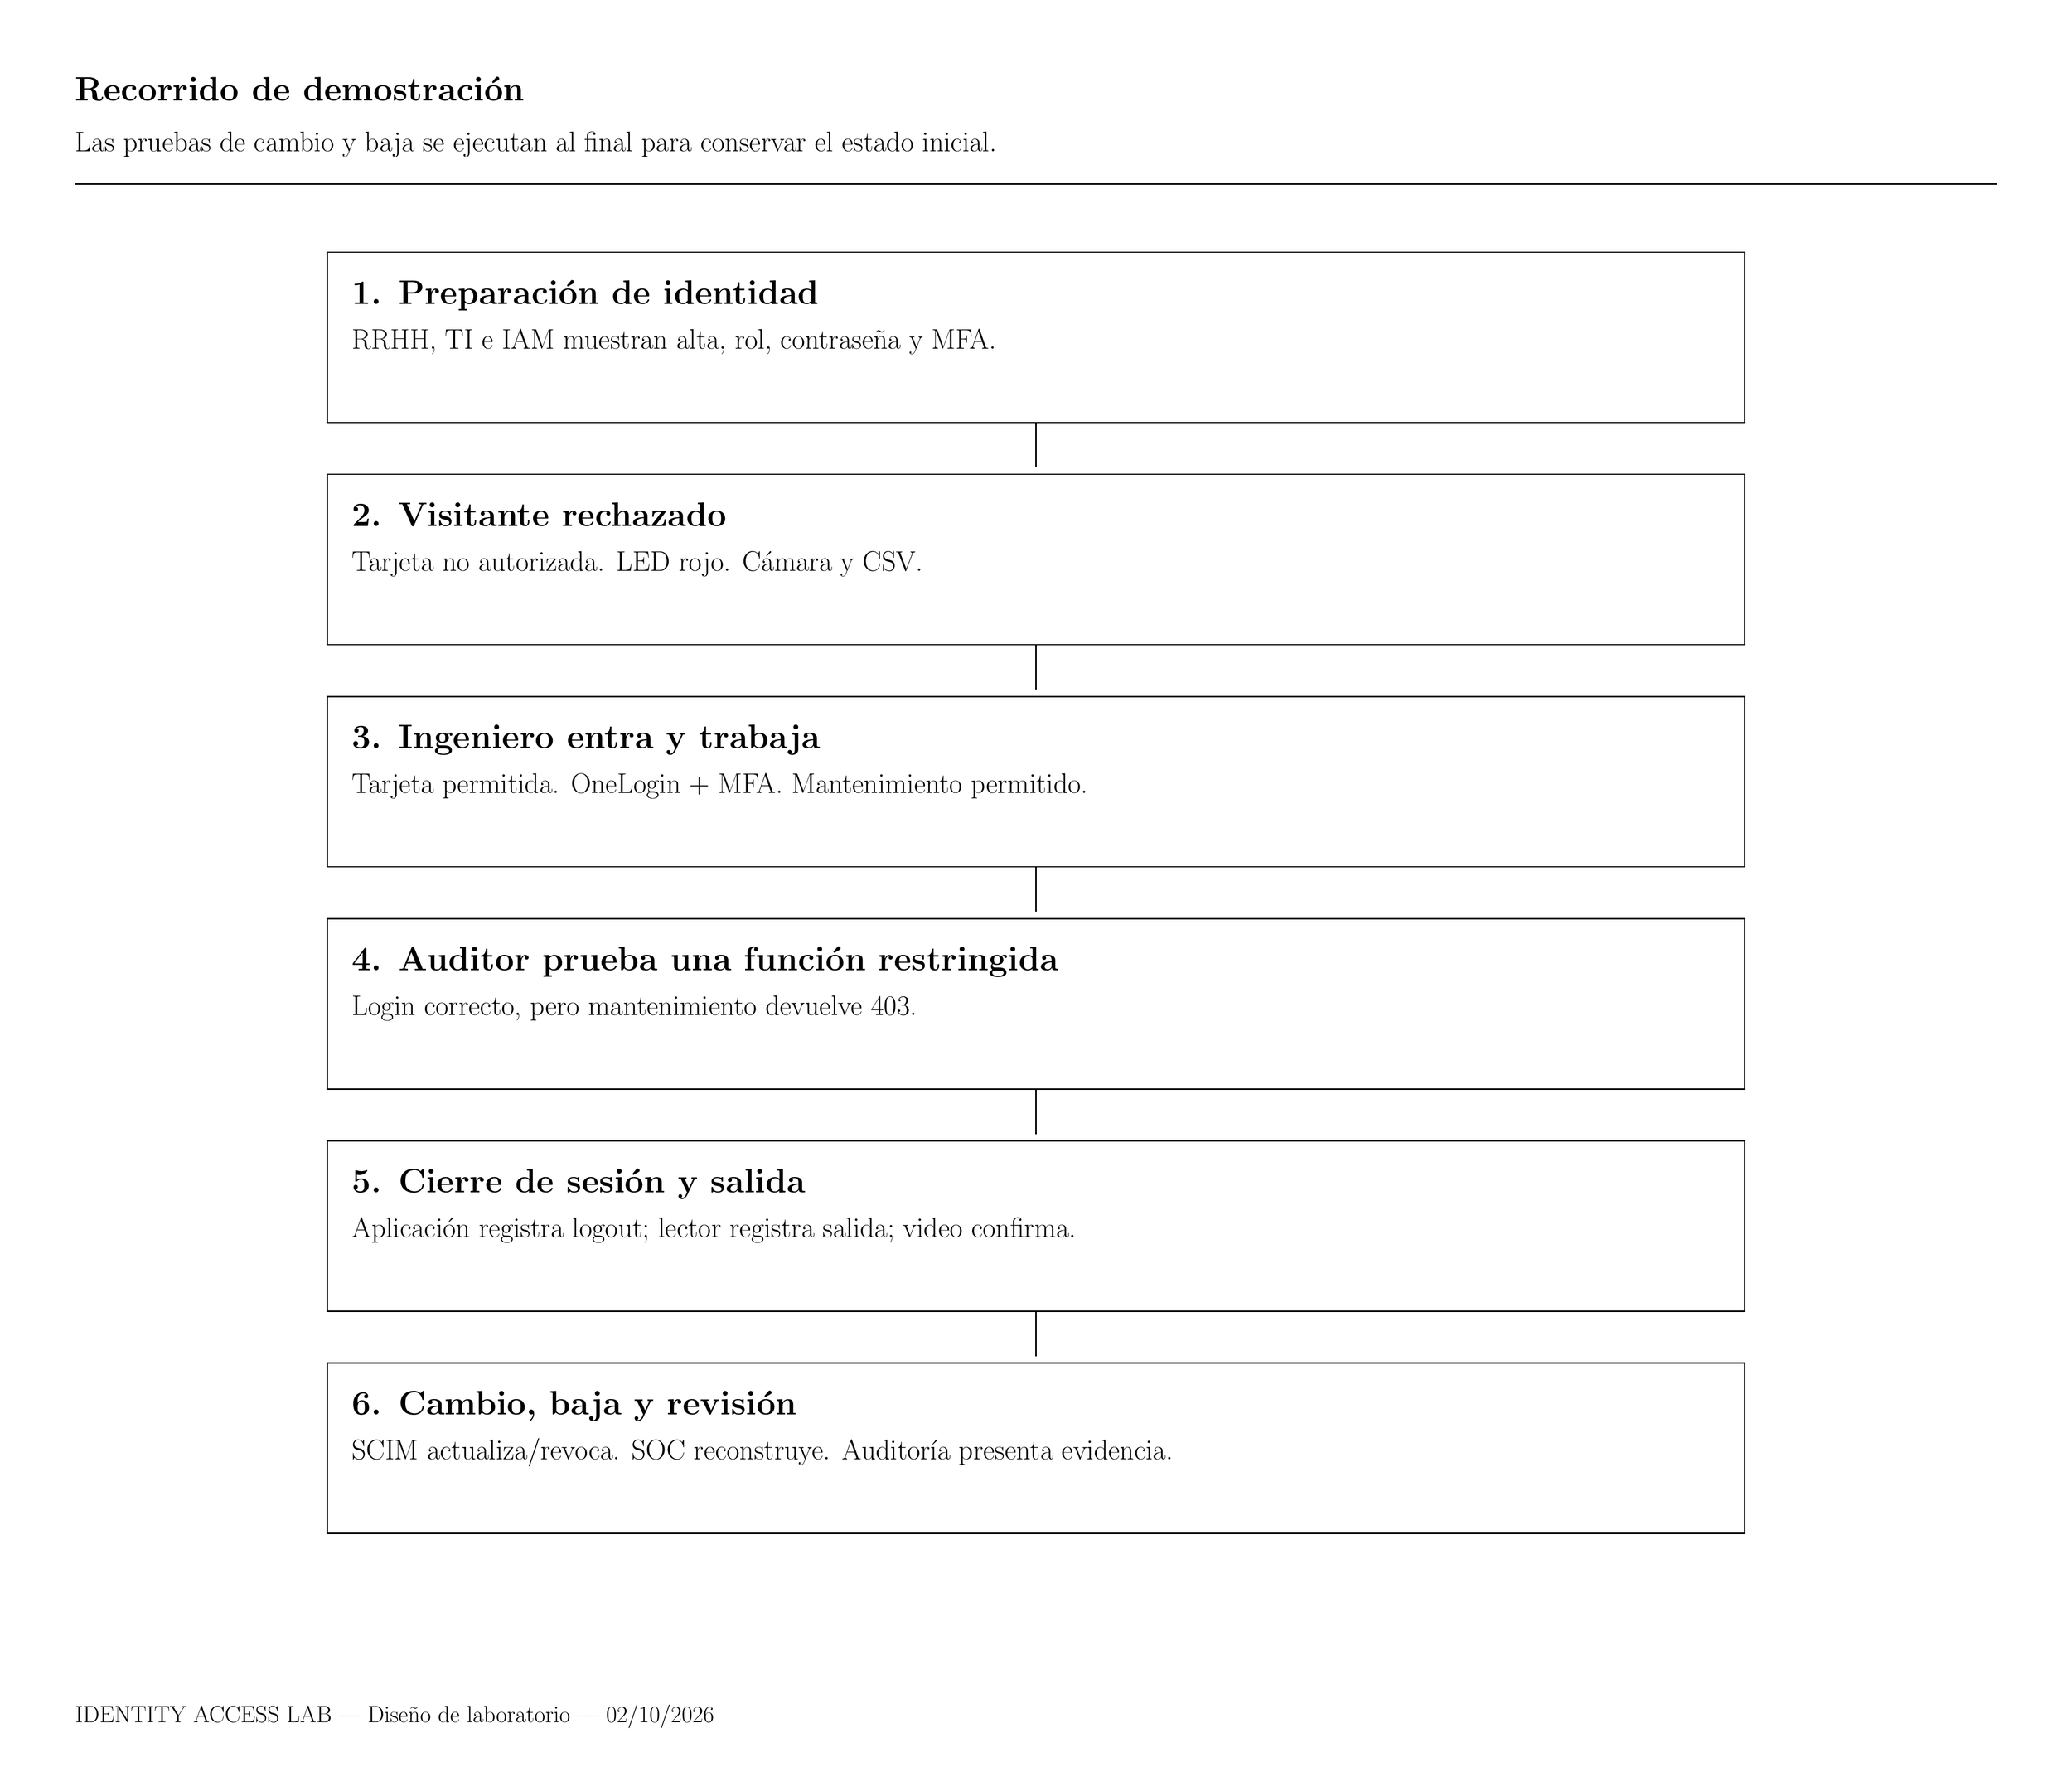
\begin{tikzpicture}[x=1pt,y=-1pt]
\path[use as bounding box] (0,0) rectangle (1500.0,1280.0);
\node[anchor=base west,inner sep=0pt,font=\fontsize{34.0}{40.8}\selectfont \bfseries ] at (45,64) {Recorrido de demostración};
\node[anchor=base west,inner sep=0pt,font=\fontsize{21.0}{25.2}\selectfont ] at (45,101) {Las pruebas de cambio y baja se ejecutan al final para conservar el estado inicial.};
\draw[line width=1pt] (45,125) -- (1455,125);
\draw[line width=1pt] (230.0,175.0) rectangle (1270.0,300.0);
\node[anchor=base west,inner sep=0pt,font=\fontsize{24.0}{28.799999999999997}\selectfont \bfseries ] at (248,213) {1. Preparación de identidad};
\node[anchor=base west,inner sep=0pt,font=\fontsize{22.0}{26.4}\selectfont ] at (248,246) {RRHH, TI e IAM muestran alta, rol, contraseña y MFA.};
\draw[line width=1pt] (750,300) -- (750,333);
\draw[line width=1pt] (230.0,338.0) rectangle (1270.0,463.0);
\node[anchor=base west,inner sep=0pt,font=\fontsize{24.0}{28.799999999999997}\selectfont \bfseries ] at (248,376) {2. Visitante rechazado};
\node[anchor=base west,inner sep=0pt,font=\fontsize{22.0}{26.4}\selectfont ] at (248,409) {Tarjeta no autorizada. LED rojo. Cámara y CSV.};
\draw[line width=1pt] (750,463) -- (750,496);
\draw[line width=1pt] (230.0,501.0) rectangle (1270.0,626.0);
\node[anchor=base west,inner sep=0pt,font=\fontsize{24.0}{28.799999999999997}\selectfont \bfseries ] at (248,539) {3. Ingeniero entra y trabaja};
\node[anchor=base west,inner sep=0pt,font=\fontsize{22.0}{26.4}\selectfont ] at (248,572) {Tarjeta permitida. OneLogin + MFA. Mantenimiento permitido.};
\draw[line width=1pt] (750,626) -- (750,659);
\draw[line width=1pt] (230.0,664.0) rectangle (1270.0,789.0);
\node[anchor=base west,inner sep=0pt,font=\fontsize{24.0}{28.799999999999997}\selectfont \bfseries ] at (248,702) {4. Auditor prueba una función restringida};
\node[anchor=base west,inner sep=0pt,font=\fontsize{22.0}{26.4}\selectfont ] at (248,735) {Login correcto, pero mantenimiento devuelve 403.};
\draw[line width=1pt] (750,789) -- (750,822);
\draw[line width=1pt] (230.0,827.0) rectangle (1270.0,952.0);
\node[anchor=base west,inner sep=0pt,font=\fontsize{24.0}{28.799999999999997}\selectfont \bfseries ] at (248,865) {5. Cierre de sesión y salida};
\node[anchor=base west,inner sep=0pt,font=\fontsize{22.0}{26.4}\selectfont ] at (248,898) {Aplicación registra logout; lector registra salida; video confirma.};
\draw[line width=1pt] (750,952) -- (750,985);
\draw[line width=1pt] (230.0,990.0) rectangle (1270.0,1115.0);
\node[anchor=base west,inner sep=0pt,font=\fontsize{24.0}{28.799999999999997}\selectfont \bfseries ] at (248,1028) {6. Cambio, baja y revisión};
\node[anchor=base west,inner sep=0pt,font=\fontsize{22.0}{26.4}\selectfont ] at (248,1061) {SCIM actualiza/revoca. SOC reconstruye. Auditoría presenta evidencia.};
\node[anchor=base west,inner sep=0pt,font=\fontsize{18.0}{21.599999999999998}\selectfont ] at (45,1254) {IDENTITY ACCESS LAB | Diseño de laboratorio | 02/10/2026};
\end{tikzpicture}}
\end{document}
